\documentclass{article}
\usepackage[utf8]{inputenc}
\usepackage[brazil]{babel}
\usepackage[a4paper, top=2.5cm, bottom=2.5cm, left=2cm, right=2.5cm, footnotesep=1.0cm]{geometry}
\usepackage{makecell}

\usepackage[sorting=none]{biblatex}
\bibliography{references}
\usepackage{csquotes}

\usepackage{hyperref}

\usepackage{amsmath,amssymb}
\newcommand*{\RandomVariable}[1]{\mathbf{#1}}
\newcommand*{\ExpectedValue}{\mathbb{E}}

\usepackage{graphicx}
\graphicspath{{figures/}}
\usepackage{subcaption}

\usepackage{pgf}
\usepackage{tikz}
\usetikzlibrary{arrows,automata,plotmarks}
\usepackage{pgfplots}
\pgfplotsset{compat=1.15}

\tikzset{
    % node styles
    state-node/.style={
        fill=none, shape=circle, draw=black, thick, text=black, minimum size=0.6cm},
    action-node/.style={
        fill=black, draw=none, text=white, shape=circle, inner sep=0.05cm, minimum size=0.2cm},
    reward-node/.style={
        fill=none, draw=black, text=black},
    hidden-node/.style={
        fill=none, draw=none, text=white, shape=circle, inner sep=0,outer sep=0, minimum size=0.0cm},
    % label styles
    action-label/.style={
        shape=circle, text=white, draw=none, fill=black, inner sep=0.05cm, minimum size=0.2cm, align=center, yshift=0.0cm, anchor=center},
    reward-label/.style={
        shape=rectangle, text=black, draw=black, fill=white, minimum size=0.5cm, align=center, yshift=0.0cm, anchor=center},
    hidden-edge/.style={
        text=white, draw=none, fill=none, inner sep=0,outer sep=0, minimum size=0.0cm},
}


% Diagrama de interação
\newcommand{\rlinteraction}{
    \begin{tikzpicture}[->,>=latex, auto, node distance=2.0cm, very thick, font=\small]
        \tikzstyle{rect-node}=[fill=none,shape=rectangle,draw=black,text=black,rounded corners=0.1cm, inner sep=0.4cm]
        \tikzstyle{hidden-node}=[fill=none, draw=none, text=black, shape=rectangle, inner sep=0,outer sep=0.05cm, minimum height=0.75cm]
        
        \node[rect-node]  (Agent)                                     {\normalsize Agent};
        \node[rect-node]  (Env)     [below of=Agent]                  {\normalsize Environment};
        \node[hidden-node] (Hidden)  [left of=Env, xshift=-0.5cm]     {};
        \node[hidden-node] (UpHid)   [above of=Hidden, yshift=-1.0cm] {};
        \node[hidden-node] (DownHid) [below of=Hidden, yshift=1.0cm]  {};
        
        \draw[thick, transform canvas={yshift=0.25cm}] (Env) to node[above] 
            {$R_{t+1}$} (Hidden);
        \draw[ultra thick, transform canvas={yshift=-0.25cm}] (Env) to node[above] 
            {$S_{t+1}$} (Hidden);
        \draw[ultra thick] (Hidden.255) to node[left, pos=1.0, yshift=1.25cm, align=center] 
            {state\\$S_t$}  ++(-1.5,0) |- (Agent.165);
        \draw[thick] (Hidden.105) to node[right, pos=1.0, yshift=0.75cm, align=center] 
            {reward\\$R_t$} ++(-1.0,0) |- (Agent.195);
        \draw[ultra thick] (Agent) to node[below right, pos=1.0, yshift=-0.5cm, align=center] 
            {action\\$A_t$} ++(3.5,0)  |- (Env);
        \draw[-, thick, dashed] (UpHid) to node {} (DownHid);
    \end{tikzpicture}
}


\newcommand{\rlinteractionpomdp}{
    \begin{tikzpicture}[->,>=latex, auto, node distance=2.0cm, very thick, font=\small]
        \tikzstyle{rect-node}=[fill=none,shape=rectangle,draw=black,text=black,rounded corners=0.1cm, inner sep=0.4cm]
        \tikzstyle{hidden-node}=[fill=none, draw=none, text=black, shape=rectangle, inner sep=0,outer sep=0.05cm, minimum height=0.75cm]
        
        \node[rect-node] (Agent) {\normalsize Agent};
        \node[rect-node] (Env) [right of=Agent, xshift=4.0cm] {\normalsize Environment};
        \node[hidden-node] (Hidden) [below of=Env, xshift=-2.0cm, yshift=0.5cm] {};
        \node[hidden-node] (UpHid) [above of=Hidden, yshift=-1.0cm] {};
        \node[hidden-node] (DownHid) [below of=Hidden, yshift=1.0cm] {};
        \node[hidden-node] (Reward) [below of=Env, xshift=0.25cm, yshift=0.5cm] {};
        
        \draw[thick, transform canvas={yshift=-0.25cm}] (Reward) to node[below, yshift=-0.1cm] 
            {$R_{t+1}$} (Hidden);
            
        \draw[ultra thick, transform canvas={xshift=0.10cm}] (Env.260) to node[xshift=-0.5cm, yshift=-0.4cm] {$O_{t+1}$} ++(0,0) |- (Hidden.105);
            
        \draw[ultra thick] (Hidden.105) to node[above, xshift=-1.5cm, align=center] 
            {observation\\$O_t$}  ++(0,0) -| (Agent.290);
        \draw[thick] (Hidden.255) to node[below, xshift=-1.5cm, align=center] 
            {reward\\$R_t$} ++(0,0) -| (Agent.250);
            
        \draw[ultra thick] (Agent) to node[xshift=3.5cm, align=center] 
            {action\\$A_t$} ++(0,1.5) -| (Env);
            
        \draw[-, thick, dashed] (UpHid) to node {} (DownHid);
    \end{tikzpicture}
}


\newcommand{\mdpthreestate}{
    \begin{tikzpicture}[->,>=stealth', auto, node distance=4.0cm, thick]
        \node[state-node]  (S1) {$s_1$};
        \node[state-node]  (S2) [below of=S1, xshift=-3.0cm] {$s_2$};
        \node[state-node]  (S3) [below of=S1, xshift= 3.0cm] {$s_3$};
        \node[action-node] (A1) [below of=S1, yshift=2.5cm, xshift=-3.0cm] {$a_1$};
        \node[action-node] (A2) [below of=S1, yshift=2.5cm]  {$a_2$};
        \node[action-node] (A3) [below of=S1, yshift=2.5cm, xshift=2.6cm] {$a_3$};
        
        \draw[bend right=20,-] (S1) to node[]  {} (A1);
        \draw[-]               (S1) to node[]  {} (A2);
        \draw[bend left=20,-] (S1) to node[]  {} (A3);
        
        \draw[bend right=30]   (A1) to node[left, pos=0.2]  {$p_1$} (S2);
        \draw[bend left=30]    (A1) to node[right, pos=0.2] {$p_2$} (S2);
        \draw[bend left=40]    (A2) to node[left, pos=0.3]  {$p_3$} (S2);
        \draw[bend right=40]   (A2) to node[right, pos=0.3] {$p_4$} (S3);
        \draw[bend left=20]    (A3) to node[right, pos=0.2] {$1$} (S3);
        
        \draw[hidden-edge, bend right=30] (A1) to node[reward-label] {$r_1$} (S2);
        \draw[hidden-edge, bend left=30]  (A1) to node[reward-label] {$r_2$} (S2);
        \draw[hidden-edge, bend left=40]  (A2) to node[reward-label] {$r_3$} (S2);
        \draw[hidden-edge, bend right=40] (A2) to node[reward-label] {$r_4$} (S3);
        \draw[hidden-edge, bend left=20]  (A3) to node[reward-label] {$r_5$} (S3);
    \end{tikzpicture}
}

\newcommand{\mdpthreestatenoprobs}{
    \begin{tikzpicture}[->,>=stealth', auto, node distance=4.0cm, thick]
        \node[state-node]  (S1) {$s_1$};
        \node[state-node]  (S2) [below of=S1, xshift=-3.0cm] {$s_2$};
        \node[state-node]  (S3) [below of=S1, xshift= 3.0cm] {$s_3$};
        \node[action-node] (A1) [below of=S1, yshift=2.5cm, xshift=-3.0cm] {$a_1$};
        \node[action-node] (A2) [below of=S1, yshift=2.5cm]  {$a_2$};
        \node[action-node] (A3) [below of=S1, yshift=2.5cm, xshift=2.6cm] {$a_3$};
        
        \draw[bend right=20,-] (S1) to node[]  {} (A1);
        \draw[-]               (S1) to node[]  {} (A2);
        \draw[bend left=20,-] (S1) to node[]  {} (A3);
        
        \draw[bend right=30] (A1) to node[reward-label] {$r_1$} (S2);
        \draw[bend left=30]  (A1) to node[reward-label] {$r_2$} (S2);
        \draw[bend left=40]  (A2) to node[reward-label] {$r_3$} (S2);
        \draw[bend right=40] (A2) to node[reward-label] {$r_4$} (S3);
        \draw[bend left=20]  (A3) to node[reward-label] {$r_5$} (S3);
    \end{tikzpicture}
}

\newcommand{\mdpbig}{
    \begin{tikzpicture}[->,>=stealth',auto,node distance=3.5cm, thick]
        \node[state-node] (S1)                     {$s_1$};
        \node[state-node] (S2) [above right of=S1] {$s_2$};
        \node[state-node] (S3) [below right of=S1, xshift=1.0cm] {$s_3$};
        \node[state-node] (S4) [below right of=S2] {$s_4$};
        \node[state-node] (S5) [right of=S4, xshift=-1.0cm]       {$s_5$};
        
        \node[action-node] (A1) [right of=S1, xshift=-2.0cm, yshift=0.5cm] {$a_1$};
        \node[action-node] (A3) [left of=S3, xshift=1.5cm, yshift=1.0cm] {$a_3$};
        \node[action-node] (A4) [below of=S4, xshift=0.75cm, yshift=2.0cm] {$a_4$};
        
        % from (S1)
        \draw[-] (S1) to node[] {} (A1);
        \draw[bend right=20] (A1) to node[left, pos=0.25] {$p_1$} (S2);
        \draw[bend left=20] (A1) to node[below, pos=0.25] {$p_2$} (S4);
        \draw[hidden-edge, bend right=20] (A1) to node[reward-label, pos=0.55] {$r_1$} (S2);
        \draw[hidden-edge, bend left=20] (A1) to node[reward-label, pos=0.60] {$r_2$} (S4);
        
        % from (S2)
        \draw[bend left=20] (S2) to node[action-label, pos=0.25] {$a_2$} (S4);
        \draw[hidden-edge, bend left=20] (S2) to node[reward-label, pos=0.65] {$r_3$} (S4);
        
        % from (S3)
        \draw[-, bend right=50] (S3) to node[] {} (A3);
        \draw[bend left=40] (A3) to node[above, pos=0.2] {$p_3$} (S1);
        \draw[bend right=40] (A3) to node[left, pos=0.3] {$p_4$} (S3);
        \draw[hidden-edge, bend left=40] (A3) to node[reward-label, pos=0.6] {$r_4$} (S1);
        \draw[hidden-edge, bend right=40] (A3) to node[reward-label, pos=0.6] {$r_5$} (S3);
        
        % from (S4)
        \draw[-] (S4) to node[] {} (A4);
        \draw[bend left=40] (A4) to node[left, pos=0.2] {$p_3$} (S3);
        \draw[bend right=40] (A4) to node[above, pos=0.25] {$p_4$} (S5);
        \draw[hidden-edge, bend left=40] (A4) to node[reward-label, left, pos=0.55] {$r_6$} (S3);
        \draw[hidden-edge, bend right=40] (A4) to node[reward-label, above right, pos=0.5] {$r_7$} (S5);
        
        % from (S5)
        \draw[bend right] (S5) to node[action-label, pos=0.25] {$a_5$} (S2);
        \draw[hidden-edge, bend right] (S5) to node[reward-label, pos=0.65] {$r_8$} (S2);
        
    \end{tikzpicture}
}


\newcommand{\simplebandit}{
    \begin{tikzpicture}[-,>=stealth', auto, node distance=1.5cm, thick]
        \node[state-node]  (SimpleBanditS1) {$s$};
        \node[reward-node] (SimpleBanditR1) [below of=SimpleBanditS1, xshift=-1.0cm] {$r$};
        \node[reward-node] (SimpleBanditR2) [below of=SimpleBanditS1, xshift=0.0cm]  {$r$};
        \node[reward-node] (SimpleBanditR3) [below of=SimpleBanditS1, xshift=1.0cm]  {$r$};
        
        \draw[bend right] (SimpleBanditS1) to node[action-label] {$a$} (SimpleBanditR1);
        \draw             (SimpleBanditS1) to node[action-label] {$a$} (SimpleBanditR2);
        \draw[bend left]  (SimpleBanditS1) to node[action-label] {$a$} (SimpleBanditR3);
    \end{tikzpicture}
}

\newcommand{\associativebandits}{
    \begin{tikzpicture}[thick]
        \node[draw=black] (AB1) {
            \begin{tikzpicture}[]
                \node[] (B1) {
                    \simplebandit
                };
                \node[right of=B1, xshift=2.0cm] (B2) {
                    \simplebandit
                };
                \node[right of=B2, xshift=2.0cm] (B3) {
                    \simplebandit
                };
                \node[right of=B3, xshift=1.0cm] (B4) {
                    $\boldsymbol{\cdots}$
                };
                \node[right of=B4, xshift=1.0cm] (B5) {
                    \simplebandit
                };
            \end{tikzpicture}
        };
        
        \node[draw=black, below of=AB1, yshift=-2.0cm] (AB2) {
            \begin{tikzpicture}[]
                \node[] (B1) {
                    \simplebandit
                };
                \node[right of=B1, xshift=2.0cm] (B2) {
                    \simplebandit
                };
                \node[right of=B2, xshift=2.0cm] (B3) {
                    \simplebandit
                };
                \node[right of=B3, xshift=1.0cm] (B4) {
                    $\boldsymbol{\cdots}$
                };
                \node[right of=B4, xshift=1.0cm] (B5) {
                    \simplebandit
                };
            \end{tikzpicture}
        };
        
        \node[below of=AB2, yshift=-1.0cm] (AB3) {
            $\Huge\vdots$
        };
    
        \node[draw=black, below of=AB3, yshift=-1.0cm] (AB4) {
            \begin{tikzpicture}[]
                \node[] (B1) {
                    \simplebandit
                };
                \node[right of=B1, xshift=2.0cm] (B2) {
                    \simplebandit
                };
                \node[right of=B2, xshift=2.0cm] (B3) {
                    \simplebandit
                };
                \node[right of=B3, xshift=1.0cm] (B4) {
                    $\boldsymbol{\cdots}$
                };
                \node[right of=B4, xshift=1.0cm] (B5) {
                    \simplebandit
                };
            \end{tikzpicture}
        };
        
        \draw[->, thick] (AB1) to node {} (AB2);
        \draw[->, thick] (AB2) to node {} (AB3);
        \draw[->, thick] (AB3) to node {} (AB4);
    \end{tikzpicture}
}

\newcommand{\fullrldiagram}{
    \begin{tikzpicture}[-,>=stealth', auto, node distance=1.5cm, thick]
        \node[state-node] (S1) {$s$};
        \node[reward-node] (R1S1) [below of=S1, xshift=-1.0cm] {$r$};
        \node[reward-node] (R2S1) [below of=S1]                {$r$};
        \node[reward-node] (R3S1) [below of=S1, xshift=1.0cm]  {$r$};
        
        \draw[bend right] (S1) to node[action-label] {$a$} (R1S1);
        \draw[]           (S1) to node[action-label] {$a$} (R2S1);
        \draw[bend left]  (S1) to node[action-label] {$a$} (R3S1);
        
        \node[state-node] (S2) [right of=S1, xshift=2.0cm] {$s$};
        \node[reward-node] (R1S2) [below of=S2, xshift=-1.0cm] {$r$};
        \node[reward-node] (R2S2) [below of=S2]                {$r$};
        \node[reward-node] (R3S2) [below of=S2, xshift=1.0cm]  {$r$};
        
        \draw[bend right] (S2) to node[action-label] {$a$} (R1S2);
        \draw[]           (S2) to node[action-label] {$a$} (R2S2);
        \draw[bend left]  (S2) to node[action-label] {$a$} (R3S2);
        
        \node[right of=S2, xshift=0.65cm, yshift=-0.75cm] (DOTS1) {
            $\boldsymbol{\cdots}$
        };
        
        \node[state-node] (S3) [right of=S2, xshift=3.0cm] {$s$};
        \node[reward-node] (R1S3) [below of=S3, xshift=-1.0cm] {$r$};
        \node[reward-node] (R2S3) [below of=S3]                {$r$};
        \node[reward-node] (R3S3) [below of=S3, xshift=1.0cm]  {$r$};
        
        \draw[bend right] (S3) to node[action-label] {$a$} (R1S3);
        \draw[]           (S3) to node[action-label] {$a$} (R2S3);
        \draw[bend left]  (S3) to node[action-label] {$a$} (R3S3);
        
        
        \node[state-node] (S4) [below of=S1, yshift=-2.0cm] {$s$};
        \node[reward-node] (R1S4) [below of=S4, xshift=-1.0cm] {$r$};
        \node[reward-node] (R2S4) [below of=S4]                {$r$};
        \node[reward-node] (R3S4) [below of=S4, xshift=1.0cm]  {$r$};
        
        \draw[bend right] (S4) to node[action-label] {$a$} (R1S4);
        \draw[]           (S4) to node[action-label] {$a$} (R2S4);
        \draw[bend left]  (S4) to node[action-label] {$a$} (R3S4);
        
        \node[state-node] (S5) [right of=S4, xshift=2.0cm] {$s$};
        \node[reward-node] (R1S5) [below of=S5, xshift=-1.0cm] {$r$};
        \node[reward-node] (R2S5) [below of=S5]                {$r$};
        \node[reward-node] (R3S5) [below of=S5, xshift=1.0cm]  {$r$};
        
        \draw[bend right] (S5) to node[action-label] {$a$} (R1S5);
        \draw[]           (S5) to node[action-label] {$a$} (R2S5);
        \draw[bend left]  (S5) to node[action-label] {$a$} (R3S5);
        
        \node[right of=S5, xshift=0.65cm, yshift=-0.75cm] (DOTS2) {$\boldsymbol{\cdots}$};
        
        \node[state-node] (S6) [right of=S5, xshift=3.0cm] {$s$};
        \node[reward-node] (R1S6) [below of=S6, xshift=-1.0cm] {$r$};
        \node[reward-node] (R2S6) [below of=S6]                {$r$};
        \node[reward-node] (R3S6) [below of=S6, xshift=1.0cm]  {$r$};
        
        \draw[bend right] (S6) to node[action-label] {$a$} (R1S6);
        \draw[]           (S6) to node[action-label] {$a$} (R2S6);
        \draw[bend left]  (S6) to node[action-label] {$a$} (R3S6);
        
        
        \draw[->, out=-90, in=90] (R1S1) to node[] {} (S5);
        \draw[->, out=-90, in=90] (R2S1) to node[] {} (S6);
        \draw[->, out=-90, in=90] (R3S1) to node[] {} (S4);
        
        \draw[->, out=-90, in=90] (R1S2) to node[] {} (DOTS2);
        \draw[->, out=-90, in=90] (R2S2) to node[] {} (S4);
        \draw[->, out=-90, in=90] (R3S2) to node[] {} (S5);
        
        \draw[->, out=-90, in=90] (R1S3) to node[] {} (S6);
        \draw[->, out=-90, in=90] (R2S3) to node[] {} (DOTS2);
        \draw[->, out=-90, in=90] (R3S3) to node[] {} (DOTS2);
        
        
        \node[below of=S4, yshift=-2.0cm] (DOTS3) {$\Huge\vdots$};
        \node[right of=DOTS3, xshift=2.0cm] (DOTS4) {$\Huge\vdots$};
        \node[right of=DOTS4, xshift=0.65cm] (DOTS5) {$\boldsymbol{\cdots}$};
        \node[right of=DOTS4, xshift=3.0cm] (DOTS6) {$\Huge\vdots$};
        
        
        \draw[->, out=-90, in=90] (R1S4) to node[] {} (DOTS4);
        \draw[->, out=-90, in=90] (R2S4) to node[] {} (DOTS3);
        \draw[->, out=-90, in=90] (R3S4) to node[] {} (DOTS5);
        
        \draw[->, out=-90, in=90] (R1S5) to node[] {} (DOTS5);
        \draw[->, out=-90, in=90] (R2S5) to node[] {} (DOTS3);
        \draw[->, out=-90, in=90] (R3S5) to node[] {} (DOTS6);
        
        \draw[->, out=-90, in=90] (R1S6) to node[] {} (DOTS4);
        \draw[->, out=-90, in=90] (R2S6) to node[] {} (DOTS4);
        \draw[->, out=-90, in=90] (R3S6) to node[] {} (DOTS5);
    \end{tikzpicture}
}


% text spacing
\linespread{1.3}
\setlength{\parindent}{4em}
\setlength{\parskip}{0.75em}


\newcommand{\todo}[1]{ --\textcolor{red}{\textbf{#1}}--}


\makeatletter
\def\@maketitle
{
    \begin{flushleft}
        \let \footnote \thanks
        {\Large \textbf{\@title} \par}
        {\large \textbf{\@author} \par}
        {\large \textit{\@date}}
    \end{flushleft}
    \par
    \vskip 1.5em
}
\makeatother


\title{Notas de estudo - Aprendizado por Reforço}
\author{Parte 01 - Introdução ao Aprendizado por Reforço}
\date{Paulo Bruno de Sousa Serafim - Out/19 - Mar/21}


\begin{document}

\maketitle

    \section{Avisos}
    
        \subsection{Bibliografia}
        
            Antes de qualquer coisa, fica o aviso: esses estudos foram quase totalmente baseados no livro de introdução ao Aprendizado por Reforço \cite{Sutton2018}
        
            \begin{center}
            \noindent\fbox{
                \parbox{40em}{
                    Richard S. Sutton and Andrew G. Barto. \textbf{Reinforcement Learning: An Introduction}. 2nd Edition. MIT Press, Cambridge, MA, 2018.
                }
            }
            \end{center}
            
            Naturalmente que consultei outras referências, mas, no geral, essas notas são notas de estudo desse livro.
            Sugiro a leitura dessas notas como uma introdução ao livro, portanto leia-o, que é gratuito.
            
            Mais ainda, por considerá-lo como uma fonte básica, não o cito explicitamente ao longo das notas, mas considere que ele é citado implicitamente em todas elas.
            Portanto, caso queira usar algum trecho encontrado aqui, na maioria dos casos, cite o livro.
            
        \subsection{Rigor matemático}
        
            Reforçando: essas notas foram feitas com o objetivo de estudos pessoais.
            Eu tentei escrevê-las em uma linguagem mais acessível para mim e certamente fui descuidado em alguns momentos com certos termos e definições.
            Dito isso, eu tento garantir um certo rigor matemático nas notas, mas não tanto.
            Por exemplo, algumas vezes posso mencionar que tal coisa foi provada como verdade e não pôr a prova ou sequer pôr uma referência a ela.
            Ou descrever algumas técnicas, mas omitir conceitos importantes, como na Seção \ref{sec:probabilidade}.
            
            Outra questão relacionada é a notação utilizada.
            Utilizo uma notação semelhante à do livro base, mas não exatamente igual.
            Apesar disso, tento manter a consistência ao longo de todas as notas.
            Caso ocorram diferenças de notação, muito provavelmente foi um equívoco meu e agradeço muito a quem puder apontá-las.
            
        \subsection{Comunicação, sugestões e críticas}
            
            Ficarei \textbf{muito} agradecido em receber qualquer feedback, em especial sugestões de melhoria, correção de erros e críticas de modo geral.
            Peço, por gentileza, que se você tiver alguma coisa para dizer, crie uma \emph{issue} no github das notas
            
            \begin{center}
                \url{https://github.com/paulobruno/RLStudyNotes} .
            \end{center}
            Caso isso não seja possível, você pode me contatar da forma como for mais conveniente: LinkedIn, e-mail ou de qualquer outra forma.
            
            
    \section{Aprendizado por Refoço}
    
        Comumente, consideramos três os paradigmas de Aprendizado de Máquina: Aprendizado Supervisionado, Aprendizado Não-Supervisionado e Aprendizado por Reforço.
        Dentre eles, o Aprendizado por Reforço é talvez o mais próximo da maneira como nós humanos construímos conhecimento, o que nos vem à mente quando pensamos em um aprendizado através da interação com o nosso ambiente.
        Diferentemente do Aprendizado Supervisionado, em que sabemos o resultado final esperado, e do Aprendizado Não-Supervisionado, cuja busca é encontrar padrões em um conjunto de dados, no Aprendizado por Reforço a construção do conhecimento se dá pela utilização da informação de um sinal positivo ou negativo dado como resposta a uma ação. 
        
        \subsection{O que é ``reforço''?}
        
            Antes de começar os estudos de Aprendizado por Reforço, vamos primeiro entender de onde vem o \emph{reforço}.
            Esse termo vem da psicologia e juntamente com o termo \emph{punição} foi introduzido no \emph{Behaviorismo}.
            Ambos são conceitos centrais do Behaviorismo e encapsulam em si a relação entre um estímulo e a sua consequência.
            Nesse sentido, a adição ou a remoção de uma recompensa faz com que a frequência de um comportamento aumente ou diminua.
        
            \subsubsection{Reforço vs. Punição}
            
                 \begin{itemize}
                     \item \textbf{Reforço}: processo em que a ocorrência de um comportamento é fortalecida por uma consequência de sua ocorrência. Portanto, aumenta a frequência do comportamento.
                     \item \textbf{Punição}: processo em que a ocorrência de um comportamento é enfraquecida por uma consequência de sua ocorrência. Portanto, diminui a frequência do comportamento.
                     \item \textbf{Positivo}: relacionado ao acréscimo ou adição de algo.
                     \item \textbf{Negativo}: relacionado à ausência ou subtração de algo.
                 \end{itemize}
                
            \subsubsection{Combinações Reforço/Punição \texorpdfstring{$\times$}{TEXT} Positivo/Negativo}
            
                Dessa forma, temos 4 combinações possíveis, que são resumidas na Tabela~\ref{tab:reforco-punicao} e ilustradas na Figura~\ref{fig:reforco-punicao}.
            
                \begin{table}[ht]
                    \centering
                    \caption{Relação entre estímulo e chance de ocorrência de um comportamento.}
                    \label{tab:reforco-punicao}
                    \begin{tabular}{|c|c|c|}
                        \hline
                         & \textbf{Positivo} & \textbf{Negativo} \\
                        \hline
                        \textbf{Reforço} & \makecell{Aumenta a chance de ocorrência do \\ comportamento pela adição de estímulo} & \makecell{Aumenta a chance de ocorrência do \\ comportamento pela remoção de estímulo} \\
                        \hline
                        \textbf{Punição} & \makecell{Diminui a chance de ocorrência do \\ comportamento pela adição de estímulo} & \makecell{Diminui a chance de ocorrência do \\ comportamento pela remoção de estímulo} \\
                        \hline
                    \end{tabular}
                \end{table}
            
                \begin{figure}[ht]
                    \centering
                    \begin{subfigure}[b]{.45\textwidth}
                        \centering
                        \raisebox{-0.5\height}{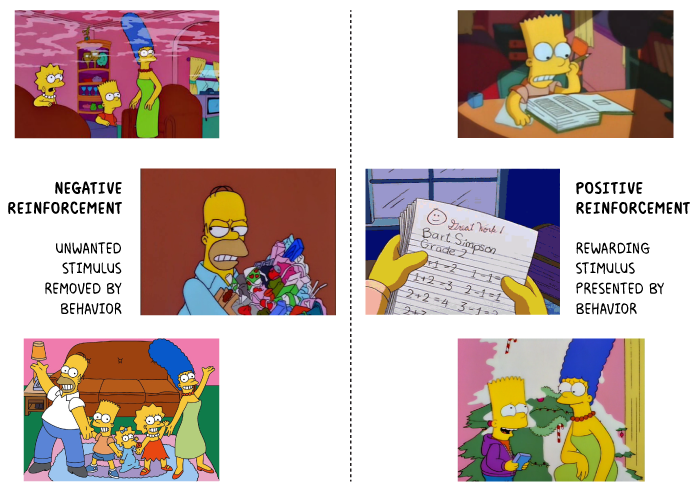
\includegraphics[width=200pt]{positive-negative-reinforcement.png}}
                        \caption{Reforço Positivo/Negativo}
                    \end{subfigure}
                    \begin{subfigure}[b]{.45\textwidth}
                        \centering
                        \raisebox{-0.5\height}{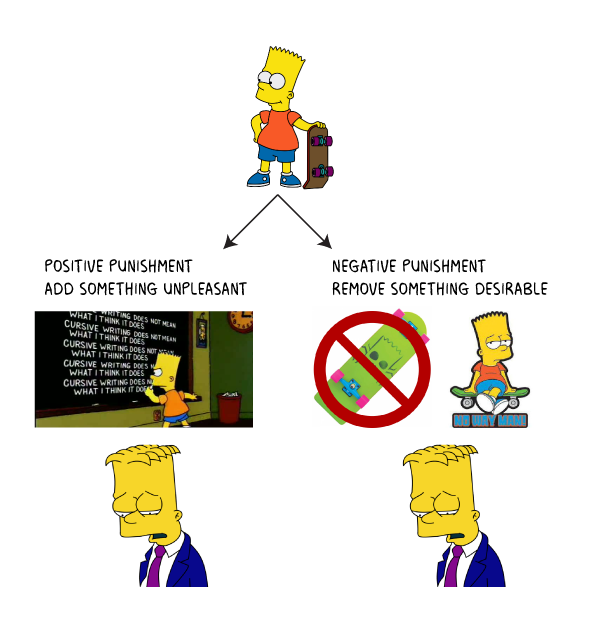
\includegraphics[width=180pt]{positive-negative-punishment_0.png}}
                        \caption{Punição Positiva/Negativa}
                    \end{subfigure}
                    \caption{Exemplos ilustrativos de reforço e punição positivas e negativas. Fonte: \citeauthor{Shrestha2017} (\citeyear{Shrestha2017}) \cite{Shrestha2017}.}
                    \label{fig:reforco-punicao}
                \end{figure}
            
    \section{Exemplos}
    
        Um exemplo tradicional é o de um cachorro que toca uma campainha, recebe um petisco e passa a tocar seguidamente para receber mais petiscos (\emph{reforço positivo}).
        Outro caso bastante conhecido, e muito utilizado pelos pais como exemplo, é o da suposta criança que pega na tomada, leva um choque e então aprende a não fazer isso novamente (\emph{punição positiva}).
        Por fim, uma situação que vai nos ajudar bastante a ilustrar o Aprendizado por Reforço, e também muito utilizado em pesquisas, é a de um jogador aprendendo a jogar um jogo qualquer.
        Claro que nós podemos extrapolar os conceitos de Aprendizado por Reforço para outras tarefas não cotidianas, como problemas de estatística, engenharia e economia.
        De modo geral, os exemplos com jogos nos ajudam a rapidamente descrever um problema e visualizar a maneira como as técnicas de Aprendizado por Reforço o resolve.
            
    \section{Características}
    
        O Aprendizado por Reforço é caracterizado pela interação entre uma entidade que executa \textbf{ações}, o \textbf{agente}, e o \textbf{ambiente} em que ela está inserida.
        Mais ainda, o agente utiliza as informações presentes no \textbf{estado} atual do ambiente.
        %, ou seja, as suas \emph{observações} do estado.
        Ocorre então um processo inerentemente sequencial de tentativa e erro, em que a melhoria do comportamento se dá de acordo com o conjunto de \textbf{recompensas} recebidas ao longo do processo, presentes e futuras, sejam elas positivas ou negativas.
        
        Podemos explicitar quatro características intrínsecas ao Aprendizado por Reforço.
        São elas:
        
        \begin{enumerate}
            \item aprendizado por tentativa e erro;
            \item problema de decisão sequencial;
            \item recompensas tardias; e
            \item aprendizado através da interação com um ambiente.
        \end{enumerate}
        
        \subsection{Aprendizado por tentativa e erro}
        
            O aprendizado por tentativa e erro é uma característica estudada na área da psicologia desde o século XIX.
            Ela está relacionada com o processo de aprendizado em que alguém executa uma ação e aprende se a ação executada foi boa ou ruim de acordo com a resposta recebida.
            Caso a resposta seja positiva, há uma tendência de que o comportamento se repita (reforço).
            Caso a resposta seja negativa, a tendência é de que o comportamento seja suprimido (punição).
        
        \subsection{Problema de decisão sequencial}
        
            Uma tarefa de Aprendizado por Reforço é um problema de decisão sequencial pois um estado só será atingido a partir de outros estados anteriores (com exceção, naturalmente, do estado inicial).
            Portanto, temos uma noção de sequência de estados percorrida pelo agente.
        
        
        \subsection{Tempo de resposta}
        
            Outra característica do Aprendizado por Reforço é a possível demora para receber uma resposta significativa.
            Por exemplo, em alguns problemas de Aprendizado por Reforço a resposta pode ser conhecida a cada iteração; já em problemas de otimização sabemos a distância para a função objetivo em todos os instantes.
            No caso do Aprendizado por Reforço, temos tarefa de recompensas imediatas e tardias.
        
            \subsubsection{Recompensas imediatas}
        
                Em algumas tarefas, recompensas significativas são recebidas após cada iteração, chamadas de \emph{recompensas imediatas}.
                Nesse caso, o agente poderá encontrar estratégias de curto prazo e ainda assim ser bem sucedido.
        
            \subsubsection{Recompensas tardias}
        
                Na maioria dos problemas, no entanto, o agente interage várias vezes com o ambiente antes de receber uma recompensa significativa.
                Recompensas tardias (do inglês \emph{delayed rewards}) referem-se ao fato de que muitas ações podem não dar nenhuma resposta significativa imediatamente, de modo que só saberemos se uma ação levou a uma sequência de eventos boa no futuro.
                Por exemplo, em um jogo de xadrez cada jogador realizará dezenas de ações antes de saber a resposta final: vitória, derrota ou empate.
                Para resolver esse tipo de problema, é necessária a descoberta de estratégias de longo prazo.
        
        \subsection{Interação com um ambiente}
    
            Diferentemente dos outros paradigmas de aprendizado, um conjunto de dados de entrada não é suficiente para o desenvolvimento dos modelos.
            No caso não-supervisionado, o objetivo é encontrar estruturas ocultas em coleções de dados, como tarefas de clusterização e redução de dimensionalidade.
            No caso supervisionado, o processo de aprendizado ocorre através de respostas instrutivas (do inglês \emph{instructive feedback}), que indicam qual a resposta esperada.
            Já no Aprendizado por Reforço, há a necessidade de que o agente interaja com um ambiente e possa ser capaz de avaliar o resultado das ações, bem como o novo estado em que se encontra. 
            
    \section{Elementos}
    
        O Aprendizado por Reforço é centrado em uma entidade que é responsável pelo processo de entender as informações disponíveis e tomar uma decisão a partir delas: o \textbf{agente}.
        No entanto, o agente não é o único elemento.
        Nas notas seguintes, entraremos em mais detalhes sobre o papel de cada um deles, bem como a formalização matemática por trás do Aprendizado por Reforço.
        Abaixo, segue uma descrição breve dos elementos mais importantes.
    
        \begin{itemize}
            \item Agente: elemento fundamental, o agente é o decisor;
            \item Ambiente: entidade que interage com o agente, direta ou indiretamente, passando informações sobre sua configuração atual e recebendo do agente as ações a serem executadas;
            \item Modelo: o conjunto de todas as informações a respeito das interações do agente com o ambiente;
            \item Política: função que retorna a probabilidade do agente executar uma ação a partir do estado atual. Na prática, a política define o comportamento do agente;
            \item Recompensa: o valor recebido pelo agente, geralmente do ambiente, após executar uma ação;
            \item Função de valor: retorna o valor esperado das recompensas totais obtidas a partir de um estado.
        \end{itemize}
        
        \subsection{Diagrama de interação}
    
            Considerando os elementos e as características dos problemas de Aprendizado por Reforço, a interação entre eles é tradicionalmente simplificada da seguinte maneira. 
            O agente. 
            Essa interação é ilustrada na Figura~\ref{diag:classical-rl}.
        
            \begin{figure}[ht]
                \centering
                \vspace*{5mm}
                \rlinteraction
                \vspace*{-5mm}
                \caption{Diagrama de interação tradicional entre os elementos. Fonte: \citeauthor{Sutton2018} (\citeyear{Sutton2018}) \cite{Sutton2018}.}
                \label{diag:classical-rl}
            \end{figure}
    
    \section{Breve história (TODO)}
    
        Três correntes separadas.
        
        \subsection{Aprendizado por tentativa e erro (learning by trial)}
        
            Ideias iniciais de aprendizado por tentativa e erro na década de 1850 por Alexander Bain;
            
            Discussão mais explícita a partir da década de 1890;
            
            Continua sendo desenvolvida pela psicologia no início do século XX;
            
            Primeiras implementações na década de 1950;
            
            Os termos “reforço” e “Aprendizado por Reforço” em problemas de tentativa e erro foram utilizados pela primeira vez na década de 1960.
        
        \subsection{Problemas de controle ótimo}
        
            Iniciado na década de 1950;
            
            Modelados como Processos de Decisão de Markov (MDP);
            
            Resolvidos através de técnicas de Programação Dinâmica.
            
            Richard Bellman (1920-1984).
            
        \subsection{Diferença temporal}
        
            Mais recente, fim dos anos 1980, com Watkins (1989);
            
            De certa forma, uniu as outras duas correntes, formando uma área só, que chamamos atualmente de Aprendizado por Reforço.
            
            Sutton and Barto, Tsisiklis and Bertsekas
            
            Tesauro's TD-Gammon (1992-1995).
        
        \subsection{Deep Reinforcement Learning}
        
            Na última década, as pesquisas em Aprendizado por Reforço receberam um novo ânimo.
            Em 2013, pesquisadores da então startup \emph{DeepMind Technologies} publicaram um artigo em que uniam um algoritmo de Aprendizado por Reforço, \emph{Q-Learning}, com o uso de \emph{Deep Neural Networks} para jogar jogos de \emph{Atari 2600}.
            Essa pesquisa resultou não somente em uma técnica nova, chamada de \emph{Deep Q-Networks} (DQN), mas também deu início a uma área de pesquisa totalmente nova: \emph{Deep Reinforcement Learning} (DRL). 
            
            Desde então, muitas pesquisas surgiram nessa área.
            Em notas futuras, falaremos mais sobre DRL.
            Nas próximas notas, no entanto, veremos conceitos elementares de Aprendizado por Reforço, de modo a conhecer as técnicas e conceitos básicos antes de avançar para os modelos mais complexos de DRL.
            Para quem tiver a curiosidade de já procurar mais sobre o assunto, listo a seguir alguns dos marcos na área.
            
            \subsubsection{Marcos \emph{recentes} utilizando DRL}
            
                \begin{itemize}
                
                    \item \textbf{2013}: Publicação no ArXiv do artigo seminal \emph{\citetitle{Mnih2013}} pela então \emph{DeepMind Technologies}, que deu início à área de \emph{Deep Reinforcement Learning} \cite{Mnih2013};
                    
                    \item \textbf{2015}: Publicação na revista \emph{Nature} do artigo \emph{\citetitle{Mnih2015}}, pelo \emph{Google DeepMind} \cite{Mnih2015};
                    
                    \item \textbf{2017}: \emph{AlphaGo} vence Lee Sedol, campão mundial de Go \cite{Silver2016,AlphaGo2017};
                    
                    \item \textbf{2019}: \emph{OpenAI Five} vence equipes campeãs mundiais do jogo Dota2 \cite{Openai2019};
                    
                    \item \textbf{2019}: AlphaStar vence dois jogadores profissionais de StarCraft II e jogadores humanos nos servidores oficias do jogo \cite{Vinyals2019}.
                    
                \end{itemize}

    \section{Brevíssima abordagem prática a alguns conceitos de Probabilidade e Estatística}
    \label{sec:probabilidade}
    
        Ao longo dos estudos, um conhecimento básico em Probabilidade e Estatística seria muito útil, mas é essencial conhecer desde o início os conceitos de \emph{valor esperado}, ou \emph{esperança}, e \emph{probabilidade condicional}.
        Por sua importância, e até mesmo simplicidade nos casos básicos, eles serão resumidamente apresentados a seguir.
        
        \textit{Nota: o objetivo dessa seção é mostrar como calcular alguns valores importantes relacionados à tomada de decisão em Aprendizado por Reforço. Por tentar ser didático e evitar falar mais conceitos do que o necessário, eu acabo sendo desleixado e não menciono conceitos extremamente importantes, como \emph{Espaço Amostral}. Peço desculpas por essa ``falha proposital'' e recomendo muito um estudo em Probabilidade e Estatística.}
            
        \subsection{Esperança}
            
            O objetivo maior em tarefas de Aprendizado por Reforço é encontrar a política que decide executar as ações cujas recompensas são máximas.
            Mais ainda, como há um conjunto de probabilidades envolvidas, desejamos executar as ações que deem a maior recompensa \emph{esperada}.
            Para calcular as recompensas esperadas, utilizaremos o conceito de \emph{valor esperado}, ou \emph{esperança}.
            
            Por exemplo, considere um dado não viciado de seis faces.
            Sabemos que podemos tirar valores de 1 a 6, mas qual é a média dos valores recebidos se jogarmos o dado várias vezes?
            
            O \emph{valor esperado} pode ser descrito como segue.
            Considere uma variável aleatória $\RandomVariable{X}$ que pode assumir $k$ valores discretos\footnote{A variável aleatória e a distribuição de probabilidade podem ser contínuas, o que é o caso frequentemente. Entretanto, ao longo das notas só veremos exemplos discretos.} $x_1$, $x_2$, \dots, $x_k$.
            De acordo com uma distribuição de probabilidade $p$, cada um desses valores ocorre com uma probabilidade $p(x_1)$, $p(x_2)$, \dots, $p(x_k)$, respectivamente.
            A \emph{esperança} (ou \emph{valor esperado}) de $\RandomVariable{X}$ sob a distribuição $p$ é definida como
            \begin{equation}
            \begin{aligned}
                \label{eq:state-value}
                \ExpectedValue_p[\RandomVariable{X}] & = \sum_{i=1}^k p(x_i) \cdot x_i \\
                & = p(x_1) \cdot x_1 + p(x_2) \cdot x_2 + \dots + p(x_k) \cdot x_k\ .
            \end{aligned}
            \end{equation}
            Para simplificar a notação, comumente o símbolo subscrito da distribuição de probabilidade $p$ é omitido, de modo que usamos somente $\ExpectedValue[\RandomVariable{X}]$.
    
            Voltando ao exemplo anterior, considere um dado de seis faces não viciado, $\RandomVariable{D}$.
            Ele pode assumir um dos valores $\{1, 2, 3, 4, 5, 6\}$, cada um deles com probabilidade $\frac{1}{6}$.
            Assim, o valor esperado de $\RandomVariable{D}$ é
            \begin{equation*}
            \begin{aligned}
                \ExpectedValue[\RandomVariable{D}] & = \frac{1}{6} \cdot 1 + \frac{1}{6} \cdot 2 + \frac{1}{6} \cdot 3 + \frac{1}{6} \cdot 4 + \frac{1}{6} \cdot 5 + \frac{1}{6} \cdot 6 \\
                & = 3.5\ .
            \end{aligned}
            \end{equation*}        
            Note que o valor esperado é a média ponderada dos valores possíveis, em que a ponderação é dada de pela distribuição de probabilidade.
            Portanto, o valor esperado de um dado não-viciado de seis faces é $3.5$.
        
        \subsection{Teorema da utilidade}
        
            Suponha que temos dois caminhos para escolher.
            Um deles é bem iluminado, com várias pessoas passando e policiamento constante.
            O outro é escuro e isolado.
            Como podemos decidir qual é o melhor caminho a seguir?
            Intuitivamente, uma pessoa ``sábia'' escolheria o primeiro, por ser mais seguro.

            Como traduzir essa intuição aos modelos de decisão?
            Primeiramente, uma vez que sabemos calcular o valor esperado de uma variável aleatória, por exemplo a recompensa esperada, essa informação pode ser útil na nossa tomada de decisão.
            Considere também que conhecemos a distribuição de probabilidades de não sofrer atentados a cada passo dado.
            Mesmo com uma visão probabilística, a pergunta continua a mesma: como podemos decidir qual é o melhor caminho a seguir?

            Em questões desse tipo, utilizaremos o \emph{teorema da utilidade máxima esperada}, de John von Neumann e Oskar Morgenstern.
            Simplificadamente, ele nos diz que entre várias opções um \emph{agente racional} (o ``sábio'' no exemplo inicial) escolherá aquela de maior valor esperado.
            Ou seja, um agente racional escolherá a opção que lhe dará potencialmente o maior resultado, em outras palavras, a opção de maior \emph{utilidade}. 
            
            Respondendo à pergunta feita anteriormente, um agente racional primeiro calcularia o valor esperado de cada caminho, como vimos nas seções anteriores, e em seguida escolheria o de maior utilidade.
            Nos estudos de Aprendizado por Reforço consideramos que o agente é sempre racional, pois o seu objetivo é obter a maior recompensa total esperada.
            
            \emph{Nota: observe que no mundo real não podemos considerar que seres humanos são agentes racionais. Muitas vezes escolhemos opções que não são ótimas por motivos pessoais. Esse é um assunto de muito estudo, por exemplo, em \emph{Teoria dos Jogos}.}
            
        \subsection{Probabilidade Condicional}
        
            Alguns eventos são independentes, ou seja, o fato de um ocorrer não interfere na chance do outro ocorrer.
            O exemplo mais tradicional é o de jogar várias moedas e observar seus resultados.
            Independentemente do primeiro resultado ter sido cara ou coroa, a probabilidade de dar coroa na segunda jogada é a mesma ($50\%$ em uma moeda não viciada).
            Outros eventos, no entanto, são dependentes de eventos anteriores.
            
            Por exemplo, considere uma loteria que me dá $1\%$ de ser vencedor.
            Observe que eu só tenho a chance de vencer se participar do sorteio.
            Caso contrário, minha chance de ganhar será $0$.
            Dessa forma, fica claro que a minha chance de vencer nessa loteria está \emph{condicionada} ao fato de participar ou não do sorteio.
            Suponha que eu participe de $80\%$ dos sorteios, qual a minha chance total de ganhar?
            
            Para responder essa pergunta, vamos utilizar o conceito de \emph{Probabilidade Condicional}.
            Seja $A$ um evento dependente de um evento $B$, a probabilidade condicional de $A$ em relação à $B$ é denotada por $P(A \mid B)$.
            Comumente, lemos $P(A \mid B)$ como ``a probabilidade de $A$ \emph{dado} $B$'', ou seja, a probabilidade do evento $A$ ocorrer, dado que o evento $B$ ocorreu.
            No exemplo anterior, seja $A = \{\text{ganhar na loteria}\}$ e $B = \{\text{participar do sorteio}\}$, $P(A | B) = 0.01$.
            
            Por definição, a probabilidade de $A$ \emph{condicionada} a $B$ é dada por
            \begin{equation}
            \label{eq:cond-prob}
            \begin{aligned}
                P(A \mid B) = \frac{P(A \cap B)}{P(B)}\ .
            \end{aligned}
            \end{equation}
            Partindo disso, podemos ver que a probabilidade de $A$ e $B$ ocorrerem simultaneamente é dada por
            \begin{equation}
            \label{eq:intersection-prob}
            \begin{aligned}
                P(A \cap B) = P(A \mid B) \cdot P(B)\ .
            \end{aligned}
            \end{equation}
            Se $A$ e $B$ são independentes, temos que
            \begin{equation*}
                P(A \cap B) = P(A) \cdot P(B)\ ,
            \end{equation*}
            logo, de \eqref{eq:cond-prob} e \eqref{eq:intersection-prob} vale também que
            \begin{equation*}
            \begin{aligned}
                P(A \mid B) & = \frac{P(A \cap B)}{P(B)}\\
                & = \frac{P(A) \cdot P(B)}{P(B)}\\
                & = P(A)\ .
            \end{aligned}
            \end{equation*}
            Analogamente, 
            \begin{equation*}
            \begin{aligned}
                P(B \mid A) & = \frac{P(B \cap A)}{P(A)}\\
                & = \frac{P(B) \cdot P(A)}{P(A)}\\
                & = P(B)\ .
            \end{aligned}
            \end{equation*}
            Para tanto, devemos ter $P(A) \neq 0$ e $P(B) \neq 0$.
            Portanto, quando $A$ e $B$ são independentes, a probabilidade de $A$ não é condicionada à probabilidade de $B$.
            Lembre que
            \begin{equation*}
                P(A \mid B) \cdot P(B) = P(A \cap B)
            \end{equation*}
            e, analogamente,
            \begin{equation*}
                P(B \mid A) \cdot P(A) = P(B \cap A)\ .
            \end{equation*}
            Ademais,
            \begin{equation*}
                P(A \cap B) = P(B \cap A)\ ,
            \end{equation*}
            portanto,
            \begin{equation*}
                P(A \mid B) \cdot P(B) = P(B \mid A) \cdot P(A)\ .
            \end{equation*}
            Rearranjando os termos, temos que
            \begin{equation}
            \label{eq:bayes}
                P(A \mid B) = \frac{P(B \mid A) \cdot P(A)}{P(B)}\ .
            \end{equation}
            A igualdade \eqref{eq:bayes}, com $P(B) \neq 0$, é conhecida como o \emph{Teorema de Bayes}.
            
            %\subsubsection{Teorema de Bayes}
            
            % PB: eu gostaria de colocar o Teorema de Bayes por uma questão de completude da nota, mas não parece necessário e pode diminuir a didática da nota.
            
            %    O Teorema de Bayes relaciona a probabilidade 
                
            \subsubsection{Lei da probabilidade total}
            
                Voltando ao exemplo do sorteio, já sabemos que $1\%$ é a probabilidade condicional de ganhar na loteria, $A$, em relação à participar do sorteio, $B$.
                Em outras palavras, se participarmos do sorteio, temos $1\%$ de chance de ganhar.
                Mas ainda não respondemos a pergunta inicial: suponha que eu participe de $80\%$ dos sorteios, qual a minha chance total de ganhar, seja participando ou não do sorteio?
                Responderemos essa questão utilizando a \emph{lei da probabilidade total}.
                
                A \emph{lei da probabilidade total} nos diz que a probabilidade total de um evento $A$ condicionada a $n$ eventos $B_n$ é dada por
                \begin{equation}
                \begin{aligned}
                    P(A) & = \sum_{n}{P(A \cap B_n)} \\
                    & = \sum_{n}{P(A \mid B_n) \cdot P(B_n)}.
                \end{aligned}
                \end{equation}
                No exemplo anterior, sejam 
                \begin{itemize}
                    \item $P(A \mid B) = 0.01$ a probabilidade de ganhar dado que participamos do sorteio,
                    \item $P(A \mid \lnot B) = 0.0$ a probabilidade de ganhar dado que não participamos do sorteio e
                    \item $P(B) = 0.8$ a probabilidade de participarmos do sorteio,
                \end{itemize}
                a probabilidade total $P(A)$ será
                \begin{equation*}
                \begin{aligned}
                    P(A) & = \sum_{n}{P(A \cap B_n)}\\
                    & = P(A \mid B) \cdot P(B) + P(A \mid \lnot B) \cdot P(\lnot B)\\
                    & = 0.01 \cdot 0.8 + 0.0 \cdot 0.2\\
                    & = 0.008\ .
                \end{aligned}
                \end{equation*}
                Ou seja, a probabilidade total de ganharmos na loteria é $0.8\%$.
                Com isso, respondemos a nossa pergunta.
            
        \subsection{União dos conceitos}
                
            Nas próximas notas, usaremos a \emph{probabilidade condicional} do \textbf{agente} executar certas \textbf{ações} no \textbf{ambiente} dado que está em um certo \textbf{estado} para calcular o \emph{valor esperado} da \textbf{recompensa} total obtida.
            Então, compararemos dois ou mais os valores esperados das recompensas totais obtidas e utilizamos o \emph{teorema da utilidade} para decidir qual é o melhor conjunto de ações a seguir, ou seja, qual é a melhor \textbf{política}, o nosso objetivo final.
            
    \printbibliography
    
\end{document}
